\documentclass[12pt,a4paper]{standalone}
\usepackage{amssymb}
\usepackage{amsmath}
\usepackage{bm}
\usepackage{tikz}
\usetikzlibrary{arrows.meta}
\usetikzlibrary{arrows}
\usepackage{pstricks}
\usetikzlibrary{patterns}
\usetikzlibrary{fadings}
\usetikzlibrary{shapes.geometric}



\begin{document}

\tikzset{every picture/.style={line width=0.75pt}} %set default line width to 0.75pt

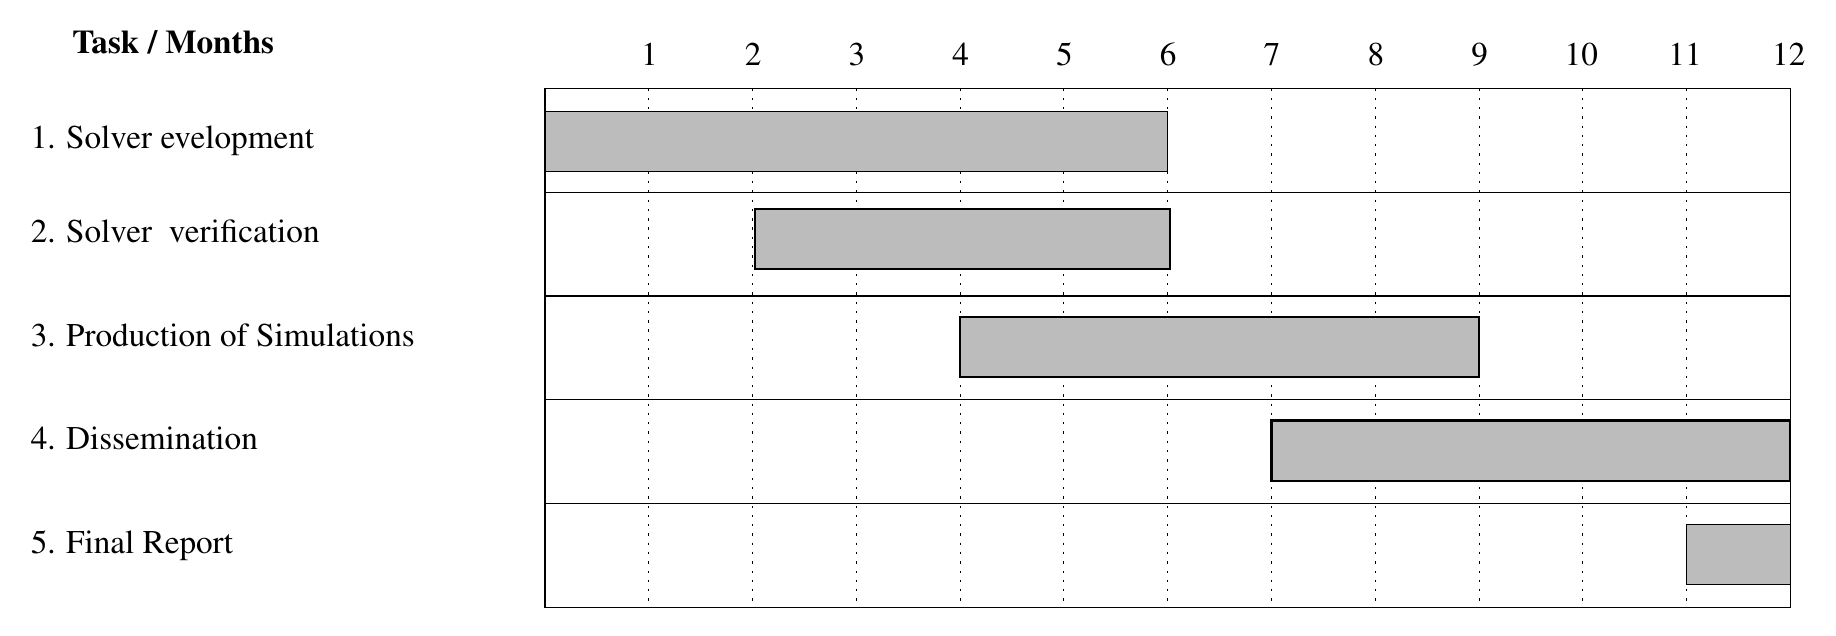
\begin{tikzpicture}[x=0.75pt,y=0.75pt,yscale=-1,xscale=1]
    %uncomment if require: \path (0,882); %set diagram left start at 0, and has height of 882

    %Shape: Grid [id:dp11237517983071033]
    \draw  [draw opacity=0][dash pattern={on 0.84pt off 2.51pt}] (300,100) -- (900,100) -- (900,350) -- (300,350) -- cycle ; \draw  [dash pattern={on 0.84pt off 2.51pt}] (350,100) -- (350,350)(400,100) -- (400,350)(450,100) -- (450,350)(500,100) -- (500,350)(550,100) -- (550,350)(600,100) -- (600,350)(650,100) -- (650,350)(700,100) -- (700,350)(750,100) -- (750,350)(800,100) -- (800,350)(850,100) -- (850,350) ; \draw  [dash pattern={on 0.84pt off 2.51pt}] (300,150) -- (900,150)(300,200) -- (900,200)(300,250) -- (900,250)(300,300) -- (900,300) ; \draw  [dash pattern={on 0.84pt off 2.51pt}] (300,100) -- (900,100) -- (900,350) -- (300,350) -- cycle ;
    %Shape: Rectangle [id:dp876104988197041]
    \draw  [color={rgb, 255:red, 0; green, 0; blue, 0 }  ,draw opacity=1 ][fill={rgb, 255:red, 188; green, 188; blue, 188 }  ,fill opacity=1 ] (300,111) -- (600,111) -- (600,140) -- (300,140) -- cycle ;
    %Shape: Rectangle [id:dp4914039708908686]
    \draw  [color={rgb, 255:red, 0; green, 0; blue, 0 }  ,draw opacity=1 ][fill={rgb, 255:red, 188; green, 188; blue, 188 }  ,fill opacity=1 ][line width=0.75]  (401,158) -- (601,158) -- (601,187) -- (401,187) -- cycle ;
    %Shape: Rectangle [id:dp2589391928032042]
    \draw  [color={rgb, 255:red, 0; green, 0; blue, 0 }  ,draw opacity=1 ][fill={rgb, 255:red, 188; green, 188; blue, 188 }  ,fill opacity=1 ][line width=0.75]  (500,210) -- (750,210) -- (750,239) -- (500,239) -- cycle ;
    %Shape: Rectangle [id:dp45296761800054064]
    \draw  [color={rgb, 255:red, 0; green, 0; blue, 0 }  ,draw opacity=1 ][fill={rgb, 255:red, 188; green, 188; blue, 188 }  ,fill opacity=1 ][line width=0.75]  (650,260) -- (900,260) -- (900,289) -- (650,289) -- cycle ;
    %Shape: Rectangle [id:dp7685593295034889]
    \draw  [color={rgb, 255:red, 0; green, 0; blue, 0 }  ,draw opacity=1 ][fill={rgb, 255:red, 188; green, 188; blue, 188 }  ,fill opacity=1 ] (850,310) -- (900,310) -- (900,339) -- (850,339) -- cycle ;
    %Shape: Rectangle [id:dp9215243929846404]
    \draw   (300,100) -- (900,100) -- (900,150) -- (300,150) -- cycle ;
    %Shape: Rectangle [id:dp2922966868335596]
    \draw   (300,150) -- (900,150) -- (900,200) -- (300,200) -- cycle ;
    %Shape: Rectangle [id:dp5463420600059313]
    \draw   (300,200) -- (900,200) -- (900,250) -- (300,250) -- cycle ;
    %Shape: Rectangle [id:dp3934008682100274]
    \draw   (300,250) -- (900,250) -- (900,300) -- (300,300) -- cycle ;
    %Shape: Rectangle [id:dp2318589337518593]
    \draw   (300,300) -- (900,300) -- (900,350) -- (300,350) -- cycle ;

    % Text Node
    \draw (345,77) node [anchor=north west][inner sep=0.75pt]   [align=left] {{\fontfamily{ptm}\selectfont {\large 1}}};
    % Text Node
    \draw (395,77) node [anchor=north west][inner sep=0.75pt]   [align=left] {{\fontfamily{ptm}\selectfont {\large 2}}};
    % Text Node
    \draw (445,77) node [anchor=north west][inner sep=0.75pt]   [align=left] {{\fontfamily{ptm}\selectfont {\large 3}}};
    % Text Node
    \draw (495,77) node [anchor=north west][inner sep=0.75pt]   [align=left] {{\fontfamily{ptm}\selectfont {\large 4}}};
    % Text Node
    \draw (545,77) node [anchor=north west][inner sep=0.75pt]   [align=left] {{\fontfamily{ptm}\selectfont {\large 5}}};
    % Text Node
    \draw (595,77) node [anchor=north west][inner sep=0.75pt]   [align=left] {{\fontfamily{ptm}\selectfont {\large 6}}};
    % Text Node
    \draw (645,77) node [anchor=north west][inner sep=0.75pt]   [align=left] {{\fontfamily{ptm}\selectfont {\large 7}}};
    % Text Node
    \draw (695,77) node [anchor=north west][inner sep=0.75pt]   [align=left] {{\fontfamily{ptm}\selectfont {\large 8}}};
    % Text Node
    \draw (745,77) node [anchor=north west][inner sep=0.75pt]   [align=left] {{\fontfamily{ptm}\selectfont {\large 9}}};
    % Text Node
    \draw (790,77) node [anchor=north west][inner sep=0.75pt]   [align=left] {{\fontfamily{ptm}\selectfont {\large 10}}};
    % Text Node
    \draw (840,77) node [anchor=north west][inner sep=0.75pt]   [align=left] {{\fontfamily{ptm}\selectfont {\large 11}}};
    % Text Node
    \draw (890,77) node [anchor=north west][inner sep=0.75pt]   [align=left] {{\fontfamily{ptm}\selectfont {\large 12}}};
    % Text Node
    \draw (71,71) node [anchor=north west][inner sep=0.75pt]   [align=left] {{\fontfamily{ptm}\selectfont {\large \textbf{Task / Months}}}};
    % Text Node
    \draw (51,117) node [anchor=north west][inner sep=0.75pt]   [align=left] {{\fontfamily{ptm}\selectfont {\large 1. Solver evelopment}}};
    % Text Node
    \draw (51,162) node [anchor=north west][inner sep=0.75pt]   [align=left] {{\fontfamily{ptm}\selectfont {\large 2. Solver \ verification}}};
    % Text Node
    \draw (51,212) node [anchor=north west][inner sep=0.75pt]   [align=left] {{\fontfamily{ptm}\selectfont {\large 3. Production of Simulations}}};
    % Text Node
    \draw (51,262) node [anchor=north west][inner sep=0.75pt]   [align=left] {{\fontfamily{ptm}\selectfont {\large 4. Dissemination}}};
    % Text Node
    \draw (51,312) node [anchor=north west][inner sep=0.75pt]   [align=left] {{\fontfamily{ptm}\selectfont {\large 5. Final Report}}};

\end{tikzpicture}

\end{document}

